\documentclass[tikz,border=10pt]{standalone}
\usepackage{amsmath}
\begin{document}
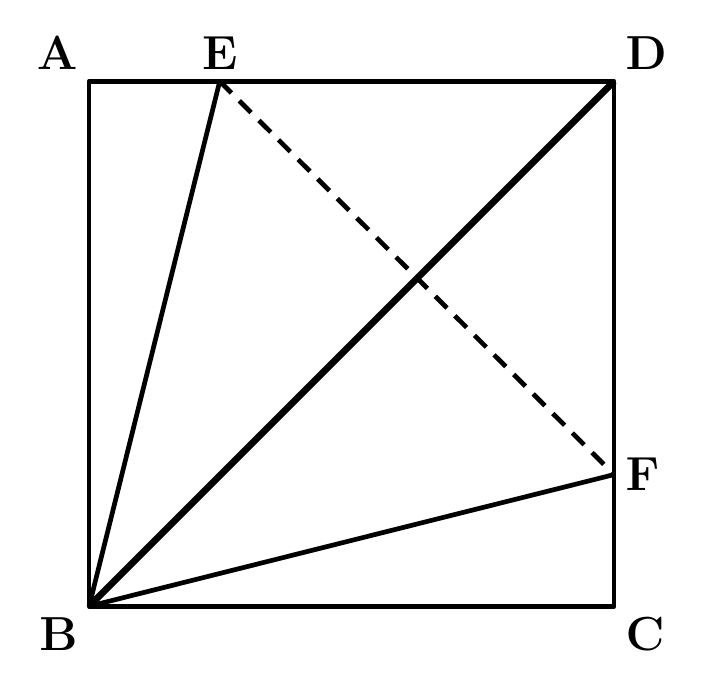
\begin{tikzpicture}[line width=1.7pt, line join=round]
% Scale s=0.021164 per px; origin at B(81,393), y up
\coordinate (B) at (0,0);
\coordinate (C) at (6.667,0);
\coordinate (D) at (6.667,6.667);
\coordinate (A) at (0,6.667);
\coordinate (E) at (1.659,6.667);   % on top edge AD
\coordinate (F) at (6.667,1.672);   % on right edge DC

% square sides
\draw (A) -- (B) -- (C) -- (D) -- cycle;
% solid diagonals to B
% diagonal DB heavier than the other spokes
\draw[line width=2.4pt] (D) -- (B);
\draw (E) -- (B);
\draw (F) -- (B);
% dashed segment E to F (crosses DB at P), longer dashes
\draw[dash pattern={on 6pt off 4pt}] (E) -- (F);

% labels (bold math, same size and positions)
\node[above left, font=\fontsize{17}{20.4}\selectfont] at (A) {$\mathbf{A}$};
\node[above right, font=\fontsize{17}{20.4}\selectfont] at (D) {$\mathbf{D}$};
\node[below right, font=\fontsize{17}{20.4}\selectfont] at (C) {$\mathbf{C}$};
\node[below left, font=\fontsize{17}{20.4}\selectfont] at (B) {$\mathbf{B}$};
\node[above, font=\fontsize{17}{20.4}\selectfont] at (E) {$\mathbf{E}$};
\node[right, font=\fontsize{17}{20.4}\selectfont] at (F) {$\mathbf{F}$};
\end{tikzpicture}
\end{document}